\section{Test Case:User-defined Atmosphere Upwelling}
%====================================================

The user-defined atmosphere test case is sightly different for that of the built-in atmosphere in that the \texttt{TAPE5} uses defined surface emissivities and reflectivities, includes CFC profile information, and invokes the FFT scanning function.

\subsection{Double precision linux results}
%------------------------------------------
The double precision results for the linux system for the user-defined atmosphere test case are shown in figure \ref{fig:run_example_user_defined_upwelling-dbl}.

\begin{figure}[htp]
  \centering
  \qquad\sffamily\textbf{Verification Example: User-defined Atmosphere Upwelling}\\
  \qquad\sffamily\textbf{Red Hat linux platform; double precision}\\
  \qquad\textsf{LBLRTM v11.3 brightness temperature difference using a locally generated TAPE3}\\
  \includegraphics[bb=85 403 534 558,clip,scale=1.0]{graphics/run_example_user_defined_upwelling/dbl.eps}
  \qquad\textsf{LBLRTM v11.3 brightness temperature difference using AER TAPE3}\\
  \includegraphics[bb=85 226 534 381,clip,scale=1.0]{graphics/run_example_user_defined_upwelling/dbl.eps}
  \caption{User-defined Atmosphere Test: Comparison of the AER-supplied \texttt{TAPE27\_ex} output to the locally generated \texttt{TAPE27} output for the \textsl{double precision} version of LBLRTM v11.3 running on a Red Hat linux system. \mbox{\textbf{(a)} Using} a locally generated little-endian \texttt{TAPE3} spectroscopic datafile. \mbox{\textbf{(b)} Using} the AER-supplied little-endian \texttt{TAPE3} spectroscopic datafile.}
  \label{fig:run_example_user_defined_upwelling-dbl}
\end{figure}

The spectral location of the main feature in the brightness temperature differences using the locally generated \texttt{TAPE3}, figure \ref{fig:run_example_user_defined_upwelling-dbl}(a), is at approximately 800\invcm{}. There are a number of water vapour lines in that region and a reasonable hypothesis for the difference is the locally generated \texttt{TAPE3} file containing more weaker water vapour lines than in the AER-supplied \texttt{TAPE3} file; presumably the creation of the latter involved some line rejection criteria.

For the case where the AER-supplied \texttt{TAPE3} is used, figure \ref{fig:run_example_user_defined_upwelling-dbl}(b), the main residual feature is an apparent sinc function centred at 937\invcm. Note that this feature also appears at the same magnitude in figure  \ref{fig:run_example_user_defined_upwelling-dbl}(a), but it is not visible due to the larger y-axis range. It would appear there is some, admittedly very small, residual, introduced into the results due to the FFT spectral reduction modules in the linux compile.


\subsection{Double precision AIX results}
%-------------------------------------------

The double precision results for the IBM AIX system for the user-defined atmosphere test case are shown in figure \ref{fig:run_example_user_defined_upwelling-dbl_ibm}.

\begin{figure}[htp]
  \centering
  \qquad\sffamily\textbf{Verification Example: User-defined Atmosphere Upwelling}\\
  \qquad\sffamily\textbf{IBM AIX platform; double precision}\\
  \qquad\textsf{LBLRTM v11.3 brightness temperature difference using a locally generated TAPE3}\\
  \includegraphics[bb=85 403 534 558,clip,scale=1.0]{graphics/run_example_user_defined_upwelling/dbl_ibm.eps}
  \qquad\textsf{LBLRTM v11.3 brightness temperature difference using AER TAPE3}\\
  \includegraphics[bb=85 226 534 381,clip,scale=1.0]{graphics/run_example_user_defined_upwelling/dbl_ibm.eps}
  \caption{User-defined Atmosphere Test: Comparison of the AER-supplied \texttt{TAPE27\_ex} output to the locally generated \texttt{TAPE27} output for the \textsl{double precision} version of LBLRTM v11.3 running on an IBM AIX system. \mbox{\textbf{(a)} Using} a locally generated big-endian \texttt{TAPE3} spectroscopic datafile. \mbox{\textbf{(b)} Using} the AER-supplied big-endian \texttt{TAPE3} spectroscopic datafile.}
  \label{fig:run_example_user_defined_upwelling-dbl_ibm}
\end{figure}

The brightness temperature differences from the run using the locally generated \texttt{TAPE3} file, figure \ref{fig:run_example_user_defined_upwelling-dbl_ibm}(a), shows the same feature as seen in  the linux system test, figure \ref{fig:run_example_user_defined_upwelling-dbl}(a).

The clear sinc function residual seen in the linux run using the AER-supplied \texttt{TAPE3} file is not present in the AIX run of figure \ref{fig:run_example_user_defined_upwelling-dbl_ibm}(b). There are other very small residual features present, but no magnification of the results indicate the presence of a residual sinc from the FFT scan function. The author is unfamiliar with that portion of the LBLRTM source code so no hypothesis as to its cause in the linux run is offered here.


\subsection{Single precision run results}
%----------------------------------------

The single precision results for both the linux and AIX systems for the user-supplied atmosphere test case are shown in figures \ref{fig:run_example_user_defined_upwelling-sgl} and \ref{fig:run_example_user_defined_upwelling-sgl_ibm} respectively.

\begin{figure}[htp]
  \centering
  \qquad\sffamily\textbf{Verification Example: User-defined Atmosphere Upwelling}\\
  \qquad\sffamily\textbf{Red Hat linux platform; single precision}\\
  \qquad\textsf{LBLRTM v11.3 brightness temperature difference using a locally generated TAPE3}\\
  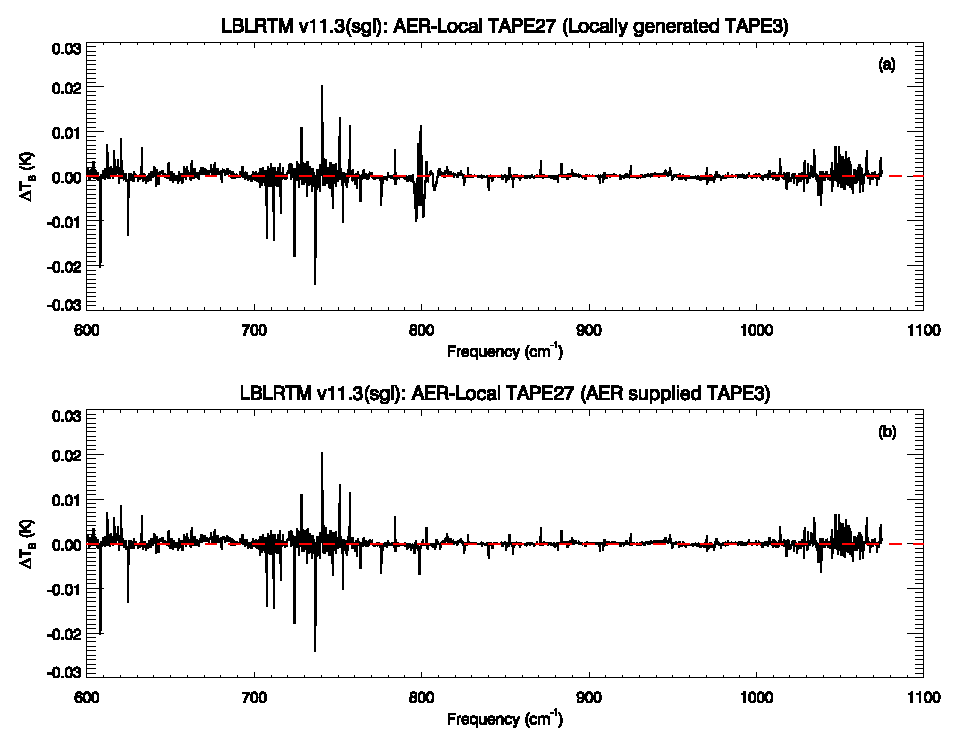
\includegraphics[bb=85 403 534 558,clip,scale=1.0]{graphics/run_example_user_defined_upwelling/sgl.eps}
  \qquad\textsf{LBLRTM v11.3 brightness temperature difference using AER TAPE3}\\
  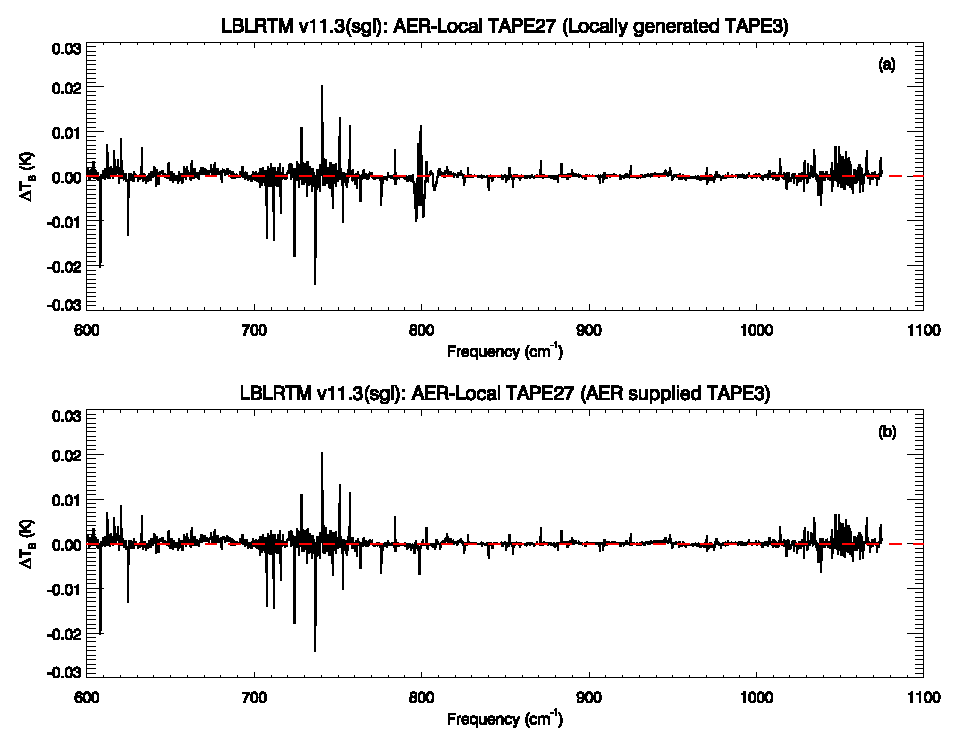
\includegraphics[bb=85 226 534 381,clip,scale=1.0]{graphics/run_example_user_defined_upwelling/sgl.eps}
  \caption{User-defined Atmosphere Test: Comparison of the AER-supplied \texttt{TAPE27\_ex} output to the locally generated \texttt{TAPE27} output for the \textsl{single precision} version of LBLRTM v11.3 running on a Red Hat linux system. \mbox{\textbf{(a)} Using} a locally generated little-endian \texttt{TAPE3} spectroscopic datafile. \mbox{\textbf{(b)} Using} the AER-supplied little-endian \texttt{TAPE3} spectroscopic datafile.}
  \label{fig:run_example_user_defined_upwelling-sgl}
\end{figure}

\begin{figure}[htp]
  \centering
  \qquad\sffamily\textbf{Verification Example: User-defined Atmosphere Upwelling}\\
  \qquad\sffamily\textbf{IBM AIX platform; single precision}\\
  \qquad\textsf{LBLRTM v11.3 brightness temperature difference using a locally generated TAPE3}\\
  \includegraphics[bb=85 403 534 558,clip,scale=1.0]{graphics/run_example_user_defined_upwelling/sgl_ibm.eps}
  \qquad\textsf{LBLRTM v11.3 brightness temperature difference using AER TAPE3}\\
  \includegraphics[bb=85 226 534 381,clip,scale=1.0]{graphics/run_example_user_defined_upwelling/sgl_ibm.eps}
  \caption{User-defined Atmosphere Test: Comparison of the AER-supplied \texttt{TAPE27\_ex} output to the locally generated \texttt{TAPE27} output for the \textsl{single precision} version of LBLRTM v11.3 running on an IBM AIX system. \mbox{\textbf{(a)} Using} a locally generated big-endian \texttt{TAPE3} spectroscopic datafile. \mbox{\textbf{(b)} Using} the AER-supplied big-endian \texttt{TAPE3} spectroscopic datafile.}
  \label{fig:run_example_user_defined_upwelling-sgl_ibm}
\end{figure}

The feature due to using the locally generated \texttt{TAPE3} file is present at around 800\invcm{} in both the linux and AIX runs. However, other than that, the two platforms yield very similar results. The character of the single precision residuals for this case are also different. Recall that the built-in atmosphere test case residuals for the single precision test case (see section \ref{sec:built_in_sgl}) indicated there was a frequency shift in the output \texttt{TAPE27} data files. That is not the case here. A magnification of figure \ref{fig:run_example_user_defined_upwelling-sgl}(b) is shown in figure \ref{fig:run_example_user_defined_upwelling-sgl_900-1000}. The character of the residuals does not indicate an issues with the \texttt{TAPE27} frequency values. This is not entirely unexpected since, if the frequency shift in the built-in atmosphere single precision test case is due to some intermediate computation at low precision, it would likely be ``removed'' -- or at least diminished -- for this test case due to the FFT scan of the high resolution result.

\begin{figure}[htp]
  \centering
  \qquad\sffamily\textbf{Verification Example: User-define Atmosphere Upwelling}\\
  \qquad\sffamily\textbf{Red Hat linux platform; single precision}\\
  \qquad\textsf{LBLRTM v11.3 brightness temperature difference using AER TAPE3}
  \includegraphics[bb=80 226 534 381,clip,scale=1.0]{graphics/run_example_user_defined_upwelling/sgl_900-1000.eps}
  \caption{User-defined Atmosphere Test: A magnification of the 900-1100\invcm{} spectral region from figure \ref{fig:run_example_user_defined_upwelling-sgl}(b). The character of the differences does not indicate a frequency shift (as seem in the figure \ref{fig:run_example_built_in_atm_upwelling-sgl_1125-1127}).}
  \label{fig:run_example_user_defined_upwelling-sgl_900-1000}
\end{figure}
